\RequirePackage{luatex85}
\documentclass{standalone}
\usepackage{tikz}
\usetikzlibrary{shapes.geometric}


\begin{document}


\begin{tikzpicture}
\node[inner sep=0pt] at (0,0){
\includegraphics[width=10cm]{./Sample_26/info_diss_sample_26_sim_100_0s_whole.pdf} };
\node[inner sep=0pt] at (0,-7){
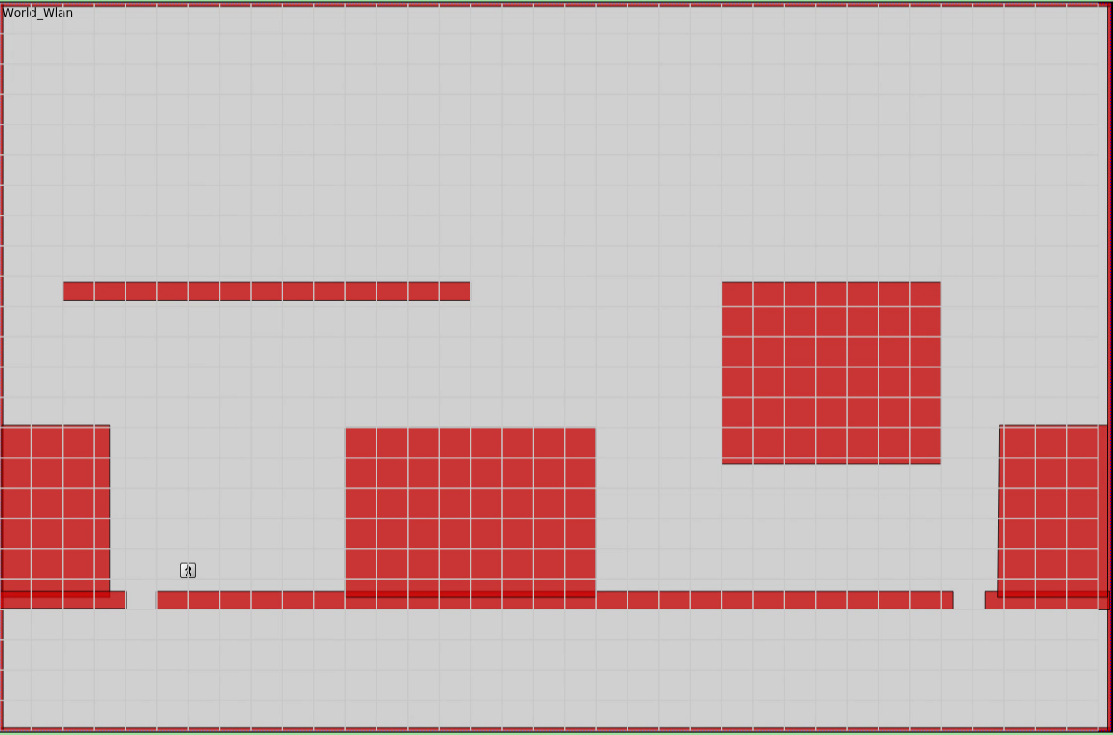
\includegraphics[width=10cm]{./Sample_26/szenarioOmnetpp.png} };
\draw[draw=purple, dashed,line width=6pt] (-5,-5.8) rectangle ++(10,2);
\node[inner sep=0pt, text width=5cm] at (0,-9.8){ Agent starting to send detour information at 100.0s};
\draw[->]  (-2.7,-9.4) -- (-3.2,-8.9);
\node[inner sep=0pt, text width=7.5cm] at (-0.5,-4.6){ Area (A1): Arrival area \\ \begin{footnotesize}
 The long walking path (left) is avoided if agents in this area are informed about the detour
\end{footnotesize} };
\node[inner sep=0pt, text width=8cm] at (0.5,1.0){ Wall (W1) };
\node[inner sep=0pt, text width=8cm] at (5.6,0.0){ Room \\ (R1) };
\node[inner sep=0pt, text width=8cm] at (-0.1,-3.0){ Closed gate };
\node[inner sep=0pt, text width=8cm] at (7.1,-3.0){ Open gate };
\draw[->]   (-3.9,-2.7) -- (-3.7,-2.3);
\draw[->]  (4,-2.7) -- (3.8,-2.4);
\draw [->] plot [smooth, tension=1] coordinates { (-4,-5.5) (-4.3,-7.1)  (0.6,-7.1) };
\draw [->] plot [smooth, tension=1] coordinates { (0,-5.5)  (1,-7) };

\end{tikzpicture}

\end{document}